% Based off of the TEMPLATE for Usenix papers (https://www.usenix.org/sites/default/files/template.la_.txt)

\documentclass[letterpaper,twocolumn,10pt]{article}
\usepackage{usenix,epsfig,endnotes,hyperref,listings,textcomp}
\usepackage[T1]{fontenc}
\usepackage{algorithm}
%\usepackage{algorithmic}
\usepackage{algpseudocode}
\lstset{
	basicstyle=\footnotesize,
	breaklines=true,
	breakatwhitespace=true,
	escapechar=\%,
	numbers=left,
	tabsize=2,
	xleftmargin=2em
}

\begin{document}

%don't want date printed
\date{\today}

%make title bold and 14 pt font (Latex default is non-bold, 16 pt)
\title{\Large \bf Time Randomization to Thwart Concurrency Bug Exploitation}

%for single author (just remove % characters)
\author{
{\rm David M. Tagatac}\\
Columbia University
%\and
%{\rm Michalis Polychronakis}\\
%Columbia University
\and
{\rm Tony Ling}\\
Columbia University
%\and
%{\rm Salvatore J. Stolfo}\\
%Columbia University
% copy the following lines to add more authors
% \and
% {\rm Name}\\
%Name Institution
} % end author

\maketitle

% Use the following at camera-ready time to suppress page numbers.
% Comment it out when you first submit the paper for review.
%\thispagestyle{empty}


\subsection*{Abstract}
TODO


\section{Introduction}
With the pervasiveness of multicore architectures, multithreading is an important - and often necessary - tool when programming for performance.  However, programming with multiple threads is generally more difficult than programming for serial execution.  Each thread has the potential to contain any bug of a serial program, and on top of that, the uncertain interleaving of concurrent threads has the potential for concurrency bugs (e.g. data races).

Lu et al. did a survey of concurrency bugs \cite{Lu2008}, and Yang et al. has demonstrated that attacks on buggy multithreaded programs are a real concern \cite{Yang2011}.  Much of the effort in combating this threat has gone into tools and systems which detect data races in order to aid debugging \cite{Savage1997, Flanagan2004, Laadan2011, Pratikakis2011, Kasikci2013}.  An alternative approach is to guide multithreaded programs into memoized synchronization schedules \cite{Cui2011}.  This approach does not dwell on race detection, but rather on removing the nondeterminism from the portions of multithreaded programs where races are most likely.  However, schedule memoization in its most automated form is still susceptible to attack whenever the attacker can trigger a different schedule by changing the input.

We address the threat of concurrency attacks from yet another angle.  Much like the way that address space layout randomization thwarts attacks that depend on absolute and/or relative code and data addresses in memory, we propose to thwart concurrency attacks that depend on specific thread timing by randomizing the delays between and among threads.  Like the memoization approach described above, we also focus on the synchronization schedule (the interleaving of the various threads in a multithreaded program).  However, instead of removing nondeterminism to increase reproducibility, we attempt to randomize the synchronization schedule to remove the possibility that the relative timing of two (or more) threads can be studied and used to craft an attack.  For this subset of concurrency attacks which depend on thread timing, we hypothesize that random injection of timing delays between concurrent threads will reduce the chance of any specific attack's success.  If such an attack can address different thread timing with correspondingly different input timing, at least randomization increases the cost to the attacker to determine the appropriate input timing; moreover, that knowledge is only useful for one system until the next randomization.

\section{Time Randomization}
Consider the following scenario: A remote attacker is communicating with some server software, and has somehow become aware of a concurrency bug in that software.  He has devised a way to exploit the bug, which includes a method for inducing a buggy thread interleaving.  For concreteness, let's assume that the bug is exposed when a save operation is attempted by one thread during the critical section of another save operation in another thread (e.g. after some checking has been done, but before the results have been used, sometimes referred to as a time of check to time of use attack).  If the server immediately spawns threads to execute save operations in response to client requests, the attacker's work consists of identifying the proper delay between two save threads such that the critical sections intersect.  The critical sections in this context are sometimes referred to as a vulnerability window \cite{Yang2011}.

If the server software is available to the attacker, he can simply study it on a similar system (which he controls) to determine the appropriate delay required to expose the bug.  Armed with this knowledge, he stands a good chance of exploiting the bug on the target system by sending requests with the same delay.

Time randomization aims to make this type of attack much harder.

\section{Experimental Design}
To test both the efficacy and the performance of time randomization as a mechanism to thwart concurrency bug exploitation, we applied time randomization to Libsafe 2.0-16.  This version of Libsafe contains a concurrency bug, for which there is a publicly available proof of concept exploit.
\subsection{CVE-2005-1125}
Libsafe is a library which protects processes against the exploitation of buffer overflow vulnerabilities in process stacks, as well as format string vulnerabilities.  It does this by intercepting all calls to C standard library functions known to be vulnerable, and then running ``safe" versions of those functions which issue warnings about exploit attempts before exiting without allowing the exploits to succeed.

A static global variable `dying' is used in Libsafe to indicate when an unsafe action has already been detected, and Libsafe is issuing warnings and exiting.  In this case, Libsafe stops checking for new exploit attempts.  However, this variable is not protected by any synchronization mechanisms, so in the case of a multithreaded program, the following sequence of events is possible:
\begin{enumerate}
	\item Thread A attempts an exploit.
	\item The exploit is caught by Libsafe, the `dying' flag is set, and Libsafe begins the warning and exit procedure.
	\item Thread B is scheduled, and attempts another exploit before Libsafe has exited thread A.
	\item Because the `dying' flag is set, thread B's exploit is not caught by Libsafe, and it succeeds.
\end{enumerate}
The proof-of-concept exploit (Figure \ref{fig_poc}) often realizes the above sequence of events, effectively bypassing Libsafe.
\begin{figure}
\lstinputlisting{libsafe-PoC.c}
\caption{The proof of concept exploit for concurrency bug CVE-2005-1125 \cite{CVE2005-1125}.  Both functions \texttt{func1} and \texttt{func2} attempt to overflow buffers in their own stack frames.  Either function running alone would be caught by Libsafe at the illegal calls to \texttt{strcpy}, but when run in parallel, the concurrency bug may allow one call to \texttt{strcpy} to succeed.}
\label{fig_poc}
\end{figure}
\subsection{Instrumentation \cite{Conrad2009}}
Time randomization was applied to Libsafe by interposing external library calls made by Libsafe each with random numbers of inline assembly NOP instructions.  This was accomplished by first specifying a max delay (per interposition).  Then, for each of the external library functions that Libsafe uses, a random integer between zero and the max delay was selected.  Finally, that number was used as the loop limit on a loop of assembly NOPs for that external library function.  The interpositions of the NOP loops were compiled into a dynamic library file, and that file was specified to be preloaded with the LD\_PRELOAD environment variable.
%TODO: add numbers of randomizations and range of maxdelay

The average time to make a (legal) \texttt{strcpy} function call, and the proof of concept exploit success rate were measured for several randomizations for each max delay ranging from 0 up to 50,000.  The dynamic library file used contains 64 external library calls made by Libsafe when the \texttt{strcpy} function is called.

\begin{algorithm}
\caption{Run Experiment}
\begin{algorithmic}[1]
\Function{run}{$max\_delay\_limit$, $iteration\_limit$, $ext\_calls$}
\State $max\_delay,iteration \gets 0$
\While{$max\_delay \leq max\_delay\_limit$}
	\While{$iteration \leq iteration\_limit$}
		\State $interpose.so \gets randomize(max\_delay)$
		\State $caught \gets repeatbug(interpose.so)$
		\State $time \gets run microbenchmark$
		\State \texttt{record $time$ and $caught$}
		\State $iteration++$
	\EndWhile
	\State $max\_delay++$
\EndWhile
\EndFunction
\State
\Function{randomize}{$delay$, $ext\_calls$}
\State $interpose.so \gets$ shared object file
\ForAll{$ext\_lib\_call$ in $ext\_calls$}
	\State create new library call $lib$
	\State insert \textbf{RAND}(0,$delay$) NOPs into $lib$
	\State insert call to $ext\_lib\_call$ into $lib$
	\State add $lib$ to $interpose.so$
\EndFor
\State \Return{$interpose.c$}
\EndFunction
\State
\Function{repeatbug}{$interpose.so$}
\State $i,count \gets 0$
\While{$i \leq 1000$}
	\State LD\_PRELOAD Libsafe and $interpose.so$
	\State run proof-of-concept show in $Figure 1$
	\If{Libsafe catches exploit}
		\State $count += 1$
	\EndIf
	\State $i++$
\EndWhile
\State \Return{$count$}
\EndFunction
\end{algorithmic}
\end{algorithm}
\subsection{Algorithm Implementation}
The psuedocode as described by Algorithm 1 explains the steps we took to introduce time randomization to Libsafe and record the overhead of each execution of the proof-of-concept code with.  To implementation this algorithm, we split up the procedure and functions into individual Python and shell scripts.

The python script run\_tests.py implements the run function, however the script does not require an $ext\_calls$ input.  $ext\_call$ is stored as func\_names.txt.  func\_names.txt is a list of all external functions to be used with this experiment.  To obtain this list, func\_names.txt starts off containing a list of all library calls in the C standard and linux/GNU specific calls as well. However, not all library calls are used by Libsafe when calling the \textbf{strcpy} function.  To filter out unused library functions, we use \textbf{ltrace} on the proof-of-concept code that uses \textbf{strcpy} to obtain a list of external functions called.  All functions not listed in this output is commented out from func\_names.txt.

By default, run\_tests.py has $max\_delay\_limit$ set to 10,0000 and $iteration\_limit$ set to 50.  Theses defaults are the parameters used for our experimentation. For 0 to $max\_delay\_limit$, a new directory is created to store the test results.  For each $max\_delay\_limit$, from 0 to $iteration\_limit$, run generate and randomize interpose.so, run repeatbug-interpose.py and run test-benchmark.sh in order.  Timing results and number of exploits caught by repeatbug-interpose.py and test-benchmark.sh is recorded for each $max\_delay$ and $iteration$.

Randomizing and generating interpose.so is done by gen\_interpose.py.  The wrapper for this script is in the makefile by using \'make random MAX\_DELAY=$max\_delay$\'.  gen\_interpose.py opens the func\_names.txt that contains the function prototypes and parses the functions.  For each uncommented out function within the list, the script constructs new a function that have the same return values, names and parameter.  The body of this new function has a loop inserted into it that executes NOPs.  The number of times it executes the NOPs is a random number choosen from 0 and $max\_delay$.  The result functions are output to interpose.so, which serves as the dynamic library that is loaded with LD\_PRELOAD.

Testing with interpose.so is done in the repeatbug-interpose.py script.  This script runs bug-interpose.so for 1000 times, and returns the amount of times the exploit is caught by Libsafe.  bug-interpose.py is uses LD\_PRELOAD to load Libsafe before interpose.so, to ensure the proof-of-concept exploit calls Libsafe functions before interpose.so functions. test-benchmark.sh is just uses LD\_PRELOAD to include Libsafe, before interpose.so as well.  It runs the baseline test and the code for this baseline testing is shown in Figure 2.



\begin{figure}
\lstinputlisting{baseline.c}
\caption{The code used for obtaining the baseline timing measurements of the proof-of-concept exploit.}
\label{fig_baseline}
\end{figure}

\section{Results}

% \begin{figure}
% \centering
% 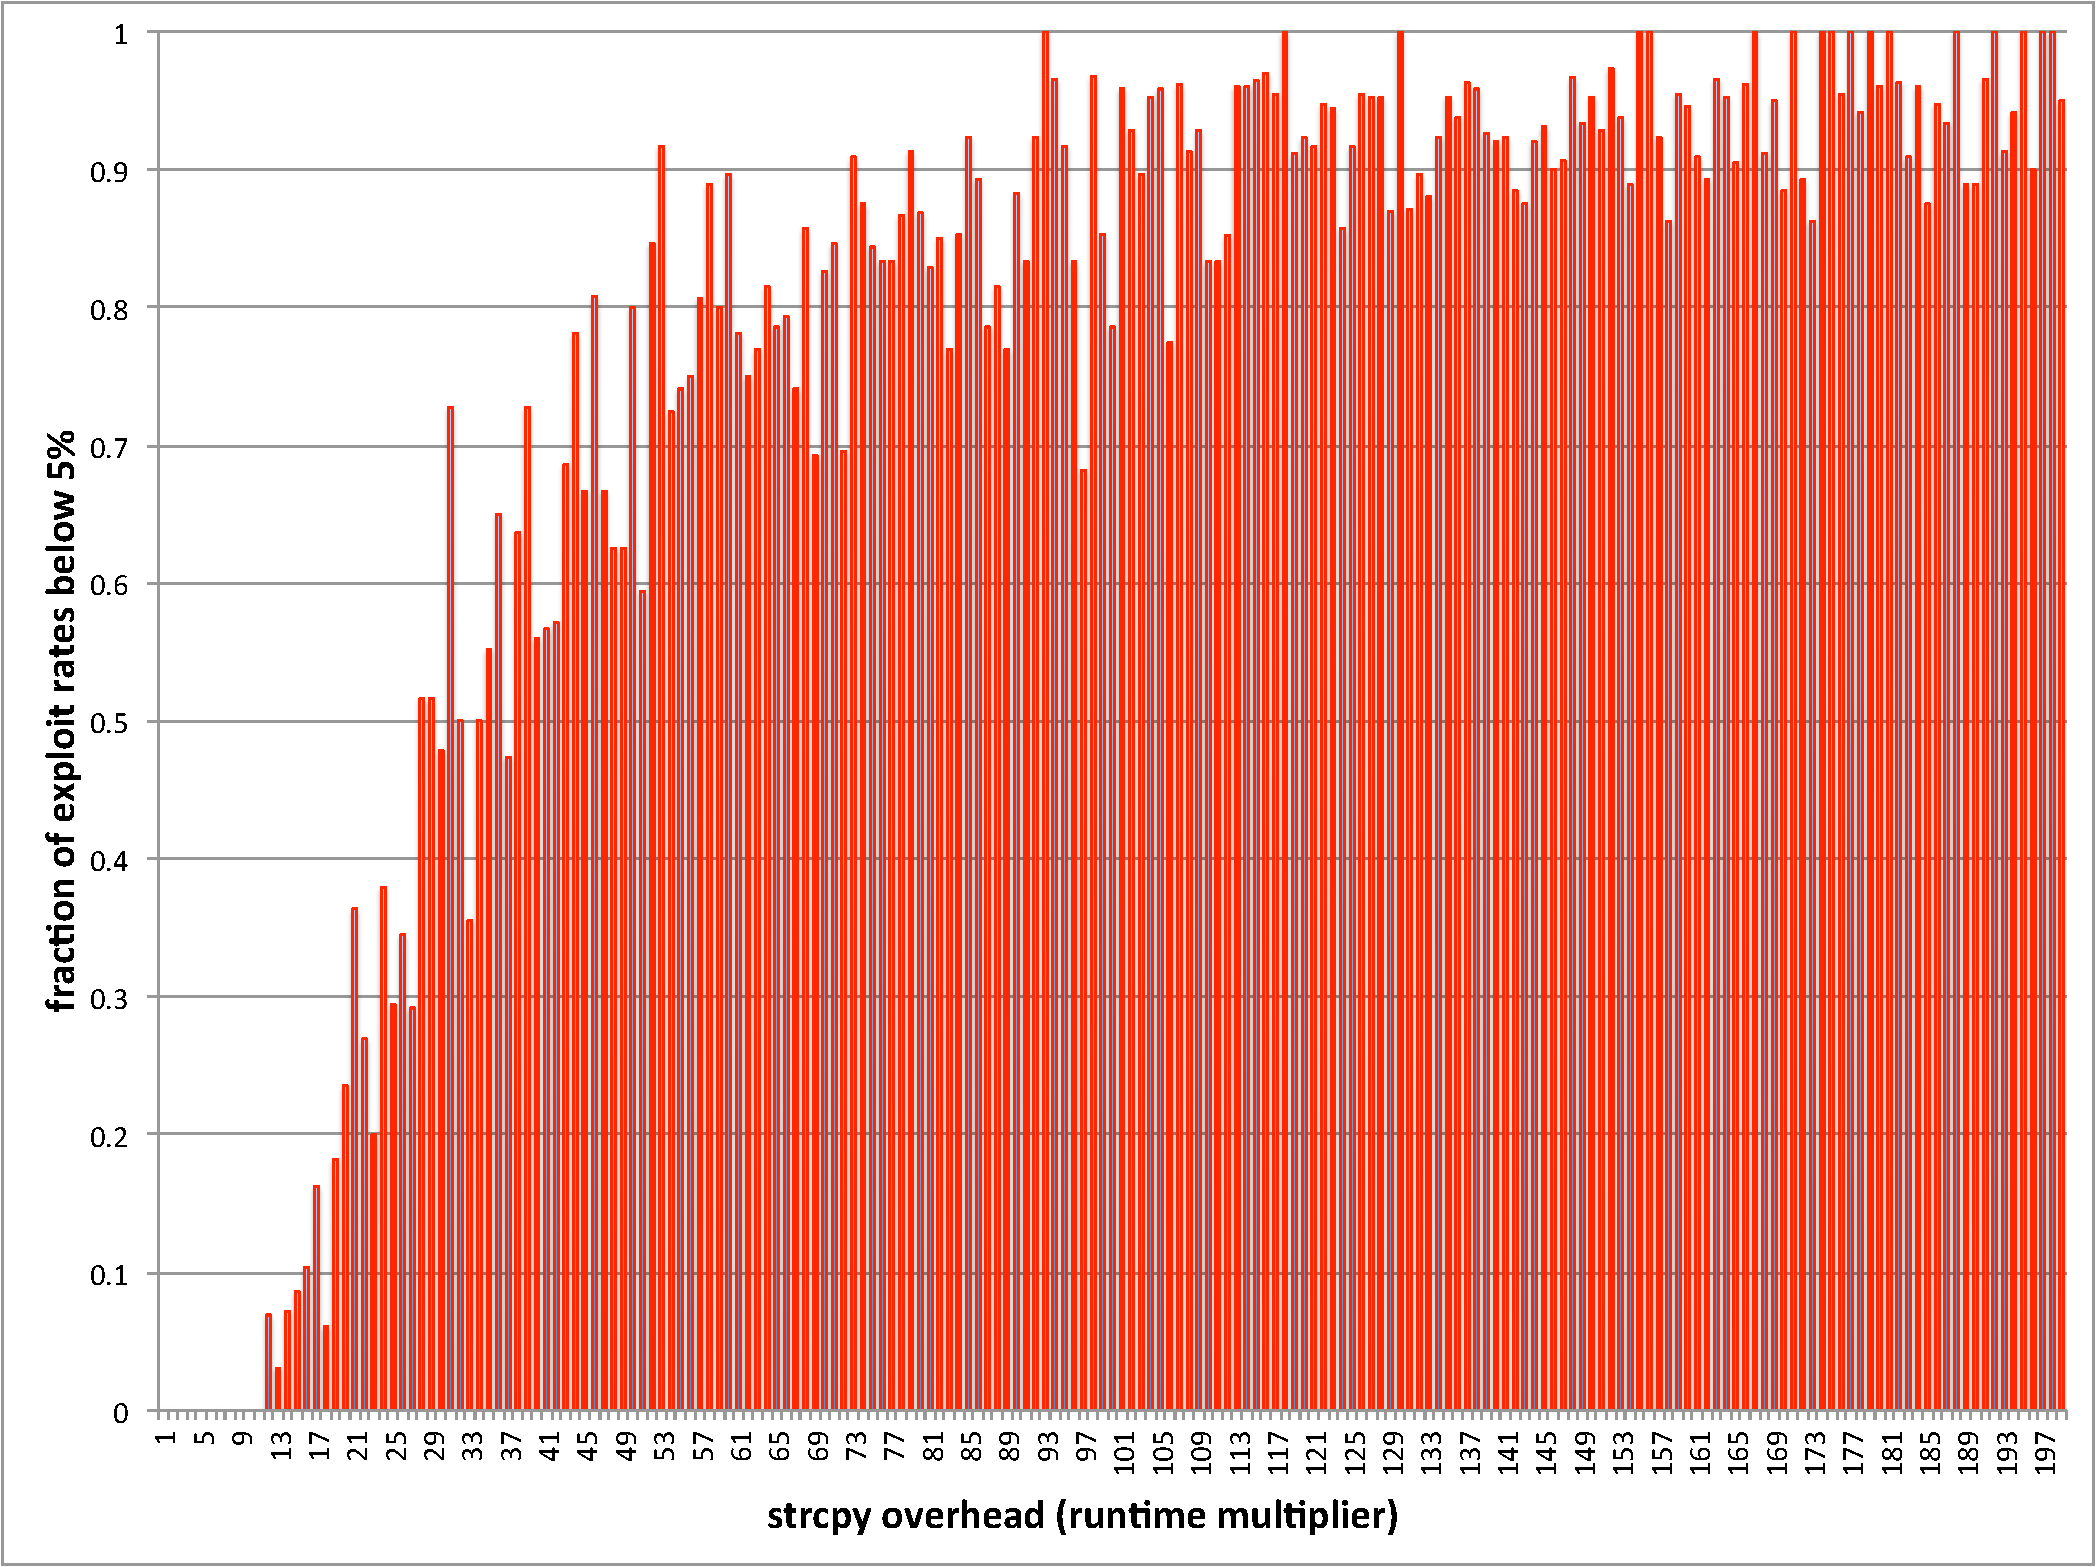
\includegraphics[width=\columnwidth]{ratefraction5.pdf}
% \caption{test}
% \label{ratefraction5}
% \end{figure}

% \begin{figure}
% \centering
% 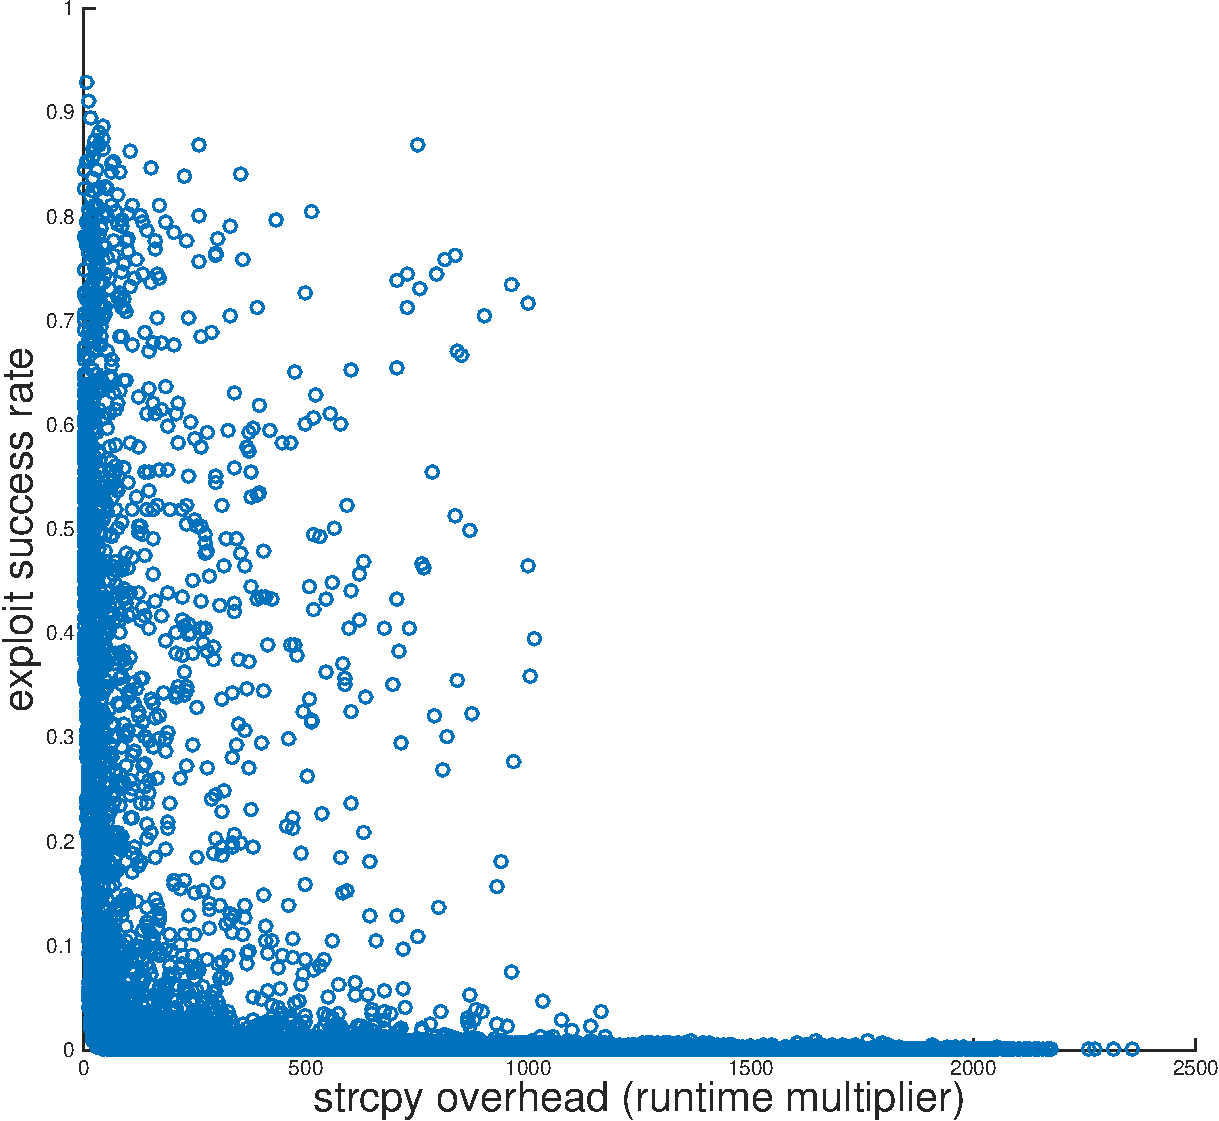
\includegraphics[width=\columnwidth]{successrate.pdf}
% \caption{test}
% \label{successrate}
% \end{figure}

% \begin{figure}
% \centering
% 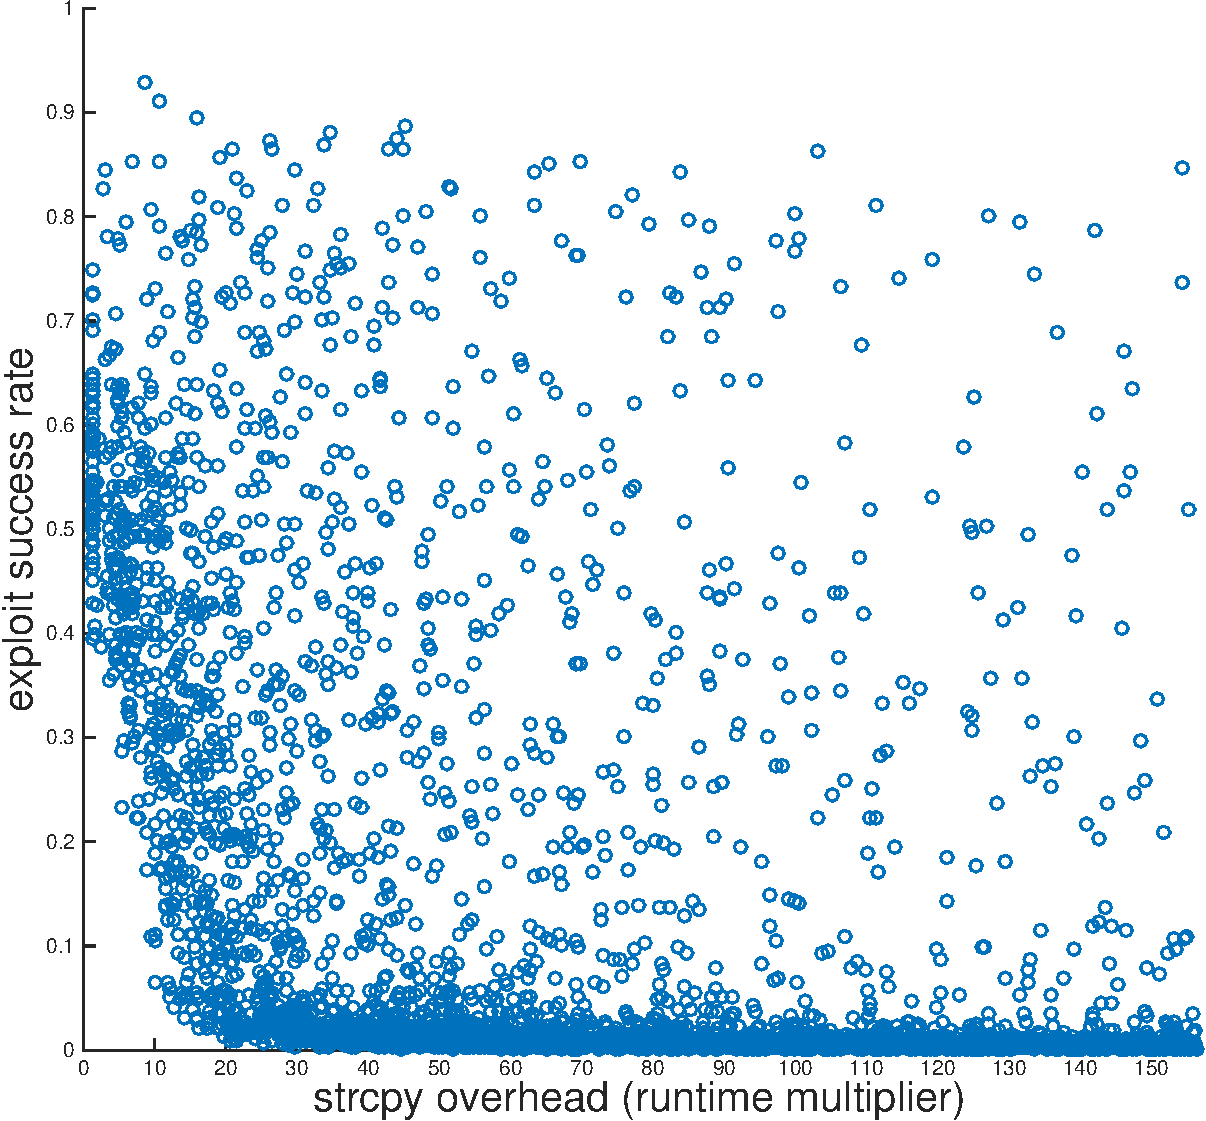
\includegraphics[width=\columnwidth]{successratezoom.pdf}
% \caption{test}
% \label{successratezoom}
% \end{figure}
The baseline results of the proof-of-concept without library interposition has a runtime of 78 ns and a 99.67\% exploit success rate.  %TODO: Add graphs and mention analysis of graphs
\section{Future Work}
The next steps are to reduce the overhead associated with time randomization.
\subsection{Heuristics}
Introducing heuristics would aid in reducing overhead of function calls.  Identifying certain functions in which time randomization have greater impact, as well as removing time randomization on functions. Instrumenting the next function call after synchronization fuctions, such as pthread library calls, is a possible heuristics.  
\subsection{Alternative Instrumentation Methods}
Alternative methods of applying time randomization might aid in reducing function overheads.  Intercepting the function calls made by the binary and introducing delays directly by injecting NOPs will remove the extra steps taken by introducing dynamic library with C code.  Modifying the scheduler is another possible route to add time delays.
\subsection{Macrobenchmarks}
This paper analyzes the proof-of-concept exploit as a microbenchmark, howerver it is important to determine exploit success rates and overhead introduced to macrobenchmarks as well. Webservers and databases, such as Apache or MySQL, would serve as good macrobenchmarks and indicators of time randomization method on actual systems.
macrobenchmarks to analyze the effects of time randomization on production or live software.
\section{Related Work}

\section{Conclusion}
Although we cannot say in the general case that time randomization is an effective method of thwarting concurrency bugs, we have demonstrated that time randomization reduce the effectiveness of the proof-of-concept exploit of CVE-2005-1125.  Further work is required to determine the effectiveness of time randomization on practical or real world systems.

Our current approach using purely random library interposition across all external function calls seems to be too costly in terms of performance.  We will need to improve this performance by implementing heuristics and exploring other methods of adding a time delay.

%\section{Preliminary Effectiveness Results}
%\begin{figure}
%\begin{lstlisting}[firstnumber=43]
%static inline long do_mmap2(
%unsigned long addr, unsigned long len,
%unsigned long prot, unsigned long flags,
%unsigned long fd, unsigned long pgoff)
%{
%	int error = -EBADF;
%	struct file * file = NULL;
%
%	flags &= ~(MAP_EXECUTABLE | MAP_DENYWRITE);
%	if (!(flags & MAP_ANONYMOUS)) {
%		file = fget(fd);
%		if (!file)
%			goto out;
%	}
%	%\textbf{udelay(100);}%
%	down_write(&current->mm->mmap_sem);
%	error = do_mmap_pgoff(file, addr, len, prot, flags, pgoff);
%	up_write(&current->mm->mmap_sem);
%
%	if (file)
%		fput(file);
%out:
%	return error;
%}
%\end{lstlisting}
%\caption{An example targeted timing delay in the CentOS Linux kernel 2.4.21 in function do\_mmap2 in arch/i386/kernel/sys\_i386.c, line 57.}
%\label{fig_mmapcode}
%\end{figure}
% \begin{figure}
% \centering
% 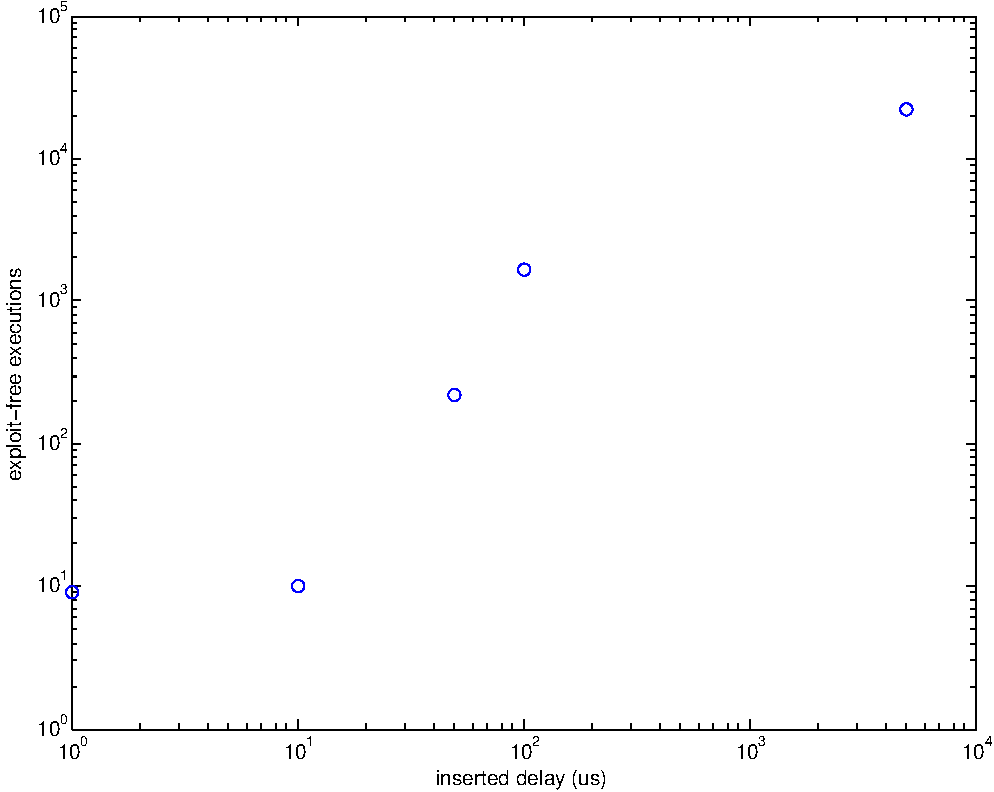
\includegraphics[width=\columnwidth]{prelimgraph}
% \caption{The effect of placing targeted timing delays in the (buggy) CentOS Linux kernel 2.4.21.  Delays between 0 and 5,000{\textmu}s were inserted strategically to alter concurrent thread timing, and the number of failed exploit script runs prior to a successful exploit strictly increased with the length of the inserted delay.}
% \label{fig_prelimgraph}
% \end{figure}
%To motivate the plausibility of our approach, we first tested the effects of targeted timing delays in buggy multithreaded code for which we have an exploit script.  The CentOS 3.9 kernel (from Linux 2.4.21) contains a critical concurrency bug that causes a system hang when exploited \cite{CVE2006-4814}.  The bug is a deadlock on the mmap semaphore `mmap\_sem' that is triggered by a specific interleaving of concurrent threads, one calling the mmap system call and the other calling the mincore system call.  The Red Hat bug report \cite{RHELbug180663} provides a script which creates two threads - one that repeatedly calls mincore in a loop, and another that repeatedly calls mmap in a loop.  By placing calls to usleep() just before the call to down\_write on mmap\_sem in the i386 architecture-specific implementation of mmap (Figure \ref{fig_mmapcode}), we were able to alter the timing of the thread interleaving.  We observed that the number of exploit script runs required for a successful exploit strictly increased with the duration of the sleep inserted (Figure \ref{fig_prelimgraph}).
%
%\section{Preliminary Performance Cost Results}
%After observing that targeted timing delays reduce the success rate of at least one concurrency bug exploit, it is relevant to ask about the performance cost of these timing delays.  I chose to run three of the core SPLASH-2 benchmarks \cite{Woo1995} as they presented the least trouble compiling on an operating system as old as CentOS 3.9.  In particular, I ran the Contiguous Partitions Ocean Simulation, the Hierarchical Radiosity Application, and the Water Simulation with Spatial Data Structure.  Each application was run three times for each delay insertion length, and then averaged to obtain the results below.
%\subsection{Ocean Simulation}
%\begin{figure}
%\centering
%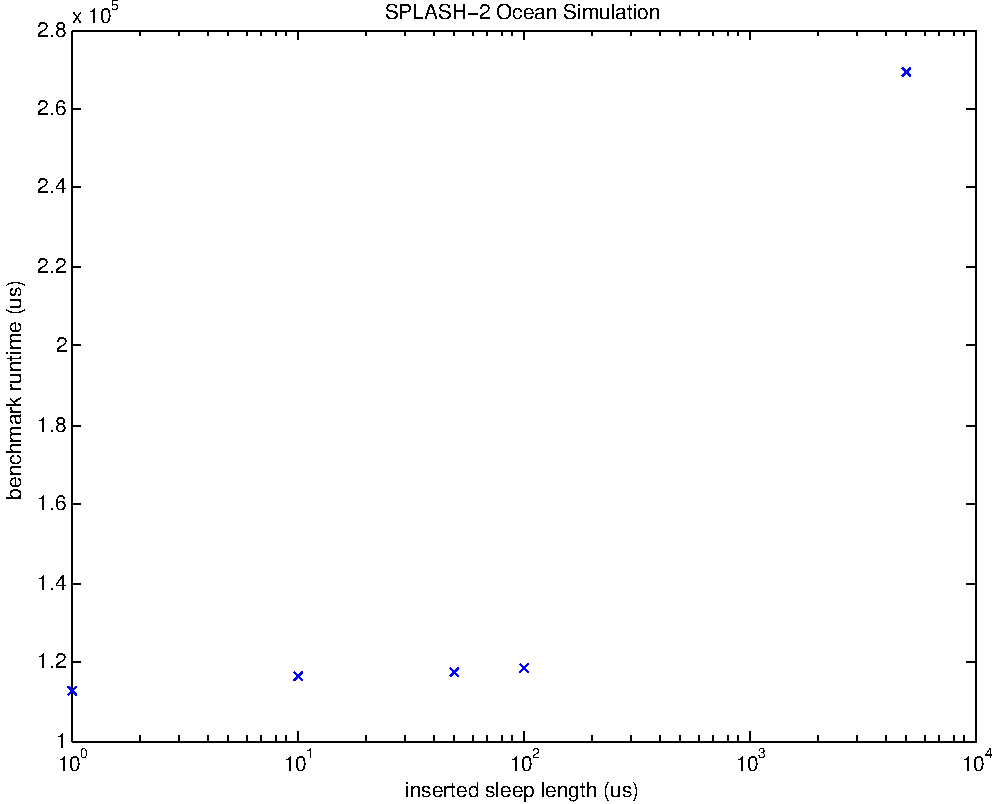
\includegraphics[width=\columnwidth]{ocean}
%\caption{The performance cost on the SPLASH-2 application OCEAN of placing targeted timing delays in the CentOS Linux kernel 2.4.21.}
%\label{fig_ocean}
%\end{figure}
%The Ocean Simulation in the SPLASH-2 benchmark suite simulates large-scale ocean movements based on eddy and boundary currents.  The Contiguous Partitions version implements the simulation grids with three-dimensional arrays.  The algorithm computes time steps of the currents in the aforementioned grids, setting up and solving spatial partial differential equations at each step \cite{Singh1992}.  I ran the simulation with the default parameters of a 258x258 grid ocean, a single processor, an error tolerance of $10^{-7}$, 20,000 meters between grid points, and 28,800 virtual seconds between timesteps.  Figure \ref{fig_ocean} shows that performance is nearly constant, increasing only slightly with the length of inserted delays, up through 100{\textmu}s.  Then with an inserted delay of 5ms, the performance takes a significant hit, running 2.36 times slower than without any inserted delay.
%\subsection{Hierarchical Radiosity}
%\begin{figure}
%\centering
%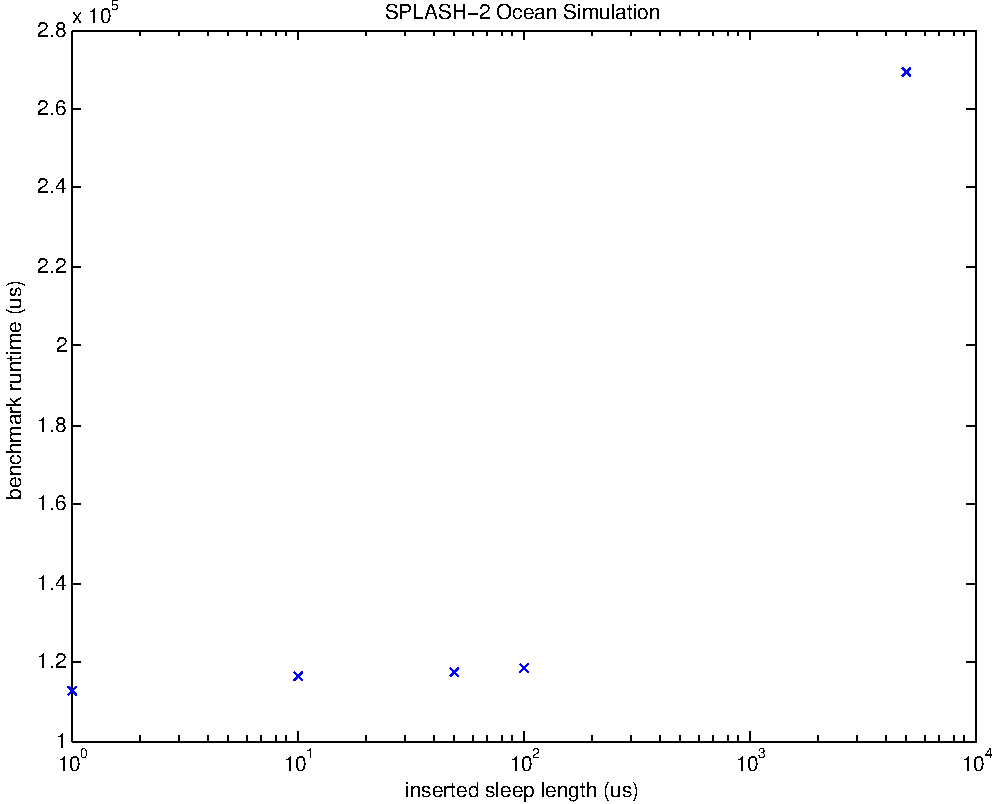
\includegraphics[width=\columnwidth]{ocean}
%\caption{The performance cost on the SPLASH-2 application RADIOSITY of placing targeted timing delays in the CentOS Linux kernel 2.4.21.}
%\label{fig_radiosity}
%\end{figure}
%The Hierarchical Radiosity Application \cite{Hanrahan1991} in SPLASH-2 quickly illuminates series of large polygonal patches, decomposing the scene into $O(n)$ blocks.  I ran this application with the room model (illumination as if the polygons are enclosed in a room), in batch mode, with a single process.  Figure \ref{fig_radiosity} shows that there is very little fluctuation in the performance of this application with respect to changes in targeted delay length.  Even with an inserted delay of 5ms, the application only sees a slowdown of less than one half of one percent.
%\subsection{Water Simulation}
%\begin{figure}
%\centering
%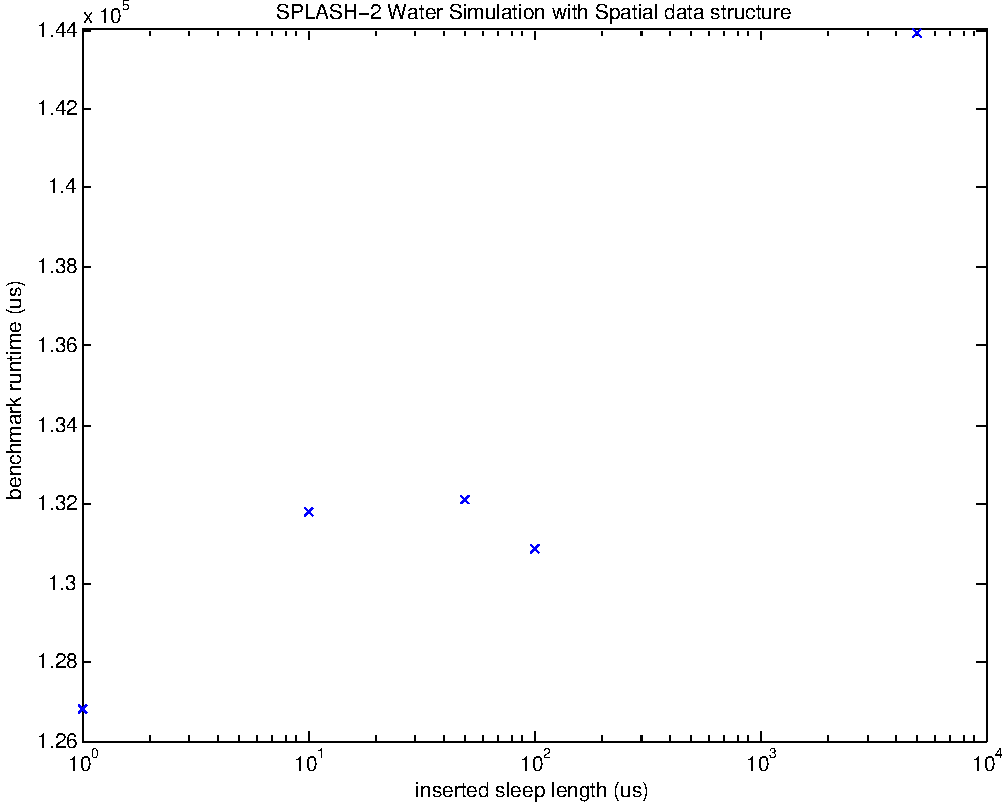
\includegraphics[width=\columnwidth]{water}
%\caption{The performance cost on the SPLASH-2 application WATER of placing targeted timing delays in the CentOS Linux kernel 2.4.21.}
%\label{fig_water}
%\end{figure}
%The Water Simulation in SPLASH-2 evaluates forces and potentials in a system of water molecules as an $n$-body problem \cite{Singh1992}.  The Spatial Data Structure algorithm approximates the solutions classically (not quantum mechanically), keeping track of the intermediary results in a 3-D spatial data structure in the cubical domain.  I used the default input parameters of $1.5 \times 10^{-16}$ seconds between timesteps, 512 molecules of water, 3 timesteps to simulate, and 1 processor.  Figure \ref{fig_water} shows a slight correlation between inserted delay in do\_mmap2 and the slowdown of the water simulation application.  With an inserted delay of 5ms, the Water Simulation experienced a 9.74\% slowdown.
%
%\section{Future Work}
%The next step is to show that randomized timing delays have a similar effect.  Our approach is to rewrite buggy multithreaded binaries, for which we have exploit scripts in hand, in the following way:
%\begin{enumerate}
%	\item Replace all function calls with jumps to variable-length NOP loops, different for each function.
%	\item At the end of these loops, jump to the originally intended function.
%	\item Randomize the NOP loop lengths on each rewrite.
%\end{enumerate}
%In this way, we can change the program timing by introducing randomness between experiments.  In a real-world scenario this would correspond to program rewrites at boot time, or some other periodic interval.  If the reduction in exploit success justifies the overhead of the timing delays, thread timing randomization could be an important defense against concurrency attacks.
%
%\section{Fennec Bug \#777045}
%Fennec, or Firefox for Mobile, contained a concurrency bug up until revision 24ed03720db7 on August 4th 2012.  This bug, when triggered, caused a doorhanger (similar to a popup) associated with one website to be displayed when viewing another website.  The bug was originally discovered by Mozilla developers running automated test suites on the Fennec code.  Specifically, the Robocop test driver, running in the talos test suite, with the test case "testCheck" - a checkerboard performance test - was shown by several developers to reproduce the bug.  It was quickly discovered that a race condition exists between the thread called to generate the doorhanger and the main thread used to display different web pages.  If the main thread "won" the race, the doorhanger could persist after its associated webpage was closed.  This appeared to be an ideal candidate for experimenting the hypothesis outlined above; however, I will now discuss the various setbacks that prevented me from even reproducing this bug, let alone randomly injecting NOPs into it.
%\subsection{Building with Clang}
%My first attempt at reproducing the bug involved trying to run testCheck in an Android emulator on my Mac.  Two things are necessary in order to run testCheck: 1) Fennec built for Android, and 2) an executable called ``xpcshell" built for the architecture that the test will run on (Darwin in this case).  However, a compatible versions of these two things were not buildable with Clang on Mac OS 10.9 at revision 3613cbdc3481 (shortly prior to the bug fix).  At first, compilation of Fennec was failing with the error message `JS\_GetNaNValue' has C-linkage specified, but returns user-defined type `jsval'.  This turned out to be because Robocop will not work with XUL Fennec - a more cross-platform-compatible version of Firefox.  However, even after building Fennec with API 14 and NDK r7c, the xpcshell binary from the Mozilla nightly builds was not compatible, failing with ``dyld: Library not loaded: @executable\_path/XUL".
%Attempts at building the same revision using Clang 3.0, targeting Darwin 9.2, with the Mac OS X 10.5 SDK, and targeting Mac OS X 10.5 also failed with the error message ``/Users/tag/Work/firefox/memory/mozjemalloc/jemalloc.c:6351:29: error: no member named `memalign' in `struct \_malloc\_zone\_t'"  Finally, after attempts to build xpcshell targeting Mac on Ubuntu 12.04 Desktop 64-but, and with some advice from some Mozilla developers, I decided to give up trying to compile with Clang, and switched to GCC.
%\subsection{Building with GCC}
%Right away, I was able to successfully build Fennec and Firefox from revision 3613cbdc3481 in an Ubuntu 12.04 VM.  However, testCheck was failing in talos with the error message talosError: ``Unable to copy `/tmp/tmpC9SIvv/profile' to remote device `/mnt/sdcard/tests/profile'".  In fact all of the talos tests were failing.  Tests were working better in the mochitest framework, but Fennec was crashing with API 14 (without GPU hardware rendering) in the Android emulator.  In fact the hardware GPU failed with APIs 14, 15, 16, and 19.
%\subsection{Real Device}
%At this point, I decided that it would be better to try on a real device, rather than continue to beat my head against the emulator, as it clearly had software graphics rendering issues.  I ordered a Samsung Galaxy Tab 2 with Android 4.1.1, rooted it with CF-AutoRoot, and installed ClockworkMod-restore.  Still mochitest-robotium failed on the device with API 14 and 16, with error message ``/sdcard/robotium.config: cannot open for write: Permission denied".  Downgrading to Android 4.0.4 (closer to the era of the bug gave more success.  In the end, I was able to get testCheck running on the device via the mochitest framework.  However, after 2,744 run, the bug was still not observed.

%{\footnotesize \bibliographystyle{acm}
%\bibliography{../common/bibliography}}
\bibliographystyle{IEEE}
\begin{thebibliography}{13}
\bibitem{Lu2008}
S. Lu, S. Park, E. Seo and Y. Zhou, ``Learning from mistakes - A Comprehensive Study on Real World Concurrency Bug Characteristics," in \emph{Proceedings of the 13th international conference on Architectural support for programming languages and operating systems} - ASPLOS XIII, New York, NY, 2008.
\bibitem{Yang2011}
J. Yang, A. Cui, S. Stolfo and S. Sethumadhavan, ``Concurrency Attacks," in HotPar'12 \emph{Proceedings of the 4th USENIX conference on Hot Topics in Parallelism}, Berkeley, CA, 2011.
\bibitem{Savage1997}
S. Savage, M. Burrows, G. Nelson, P. Sobalvarro and T. Anderson, ``Eraser: a dynamic data race detector for multithreaded programs," \emph{ACM Transactions on Computer Systems}, vol. 15, no. 4, pp. 391-411, 1997.
\bibitem{Flanagan2004}
C. Flanagan and S. N. Freund, ``Atomizer: a dynamic atomicity checker for multithreaded programs," in \emph{18th International Parallel and Distributed Processing Symposium}, 2004. Proceedings., 2004.
\bibitem{Laadan2011}
O. Laadan, C.-C. Tsai, N. Viennot, C. Blinn, P. S. Du, J. Yang and J. Nieh, ``Finding Concurrency Errors in Sequential Code—OS-level, In-vivo Model Checking of Process Races," in \emph{Proceedings of the 13th USENIX conference on Hot topics in operating systems}, 2011.
\bibitem{Pratikakis2011}
P. Pratikakis, J. S. Foster and M. Hicks, ``LOCKSMITH: Practical Static Race Detection for C," \emph{ACM Transactions on Programming Languages and Systems}, vol. 33, no. 1, pp. 1-55, 2011.
\bibitem{Kasikci2013}
B. Kasikci, C. Zamfir and G. Candea, ``RaceMob: Crowdsourced Data Race Detection," in \emph{Proceedings of the Twenty-Fourth ACM Symposium on Operating Systems Principles} - SOSP '13, New York, NY, 2013.
\bibitem{Cui2011}
H. Cui, J. Wu, J. Gallagher, H. Guo and J. Yang, ``Efficient Deterministic Multithreading through Schedule Relaxation," in \emph{Proceedings of the TwentyThird ACM Symposium on Operating Systems Principles} SOSP 11, 2011.
\bibitem{CVE2005-1125}
CVE-2005-1125. \url{http://www.cvedetails.com/cve/CVE-2005-1125/}
\bibitem{CVE2006-4814}
CVE-2006-4814. \url{http://www.cvedetails.com/cve/CVE-2006-4814/}
\bibitem{RHELbug180663}
Red Hat Bugzilla --- Bug 180663.\\\url{https://bugzilla.redhat.com/show_bug.cgi?id=180663}
\bibitem{Woo1995}
Woo, Steven Cameron, et al. ``The SPLASH-2 programs: Characterization and methodological considerations." \emph{ACM SIGARCH Computer Architecture News}, Vol. 23. No. 2. ACM, 1995.
\bibitem{Singh1992}
Singh, Jaswinder Pal, Wolf-Dietrich Weber, and Anoop Gupta. ``SPLASH: Stanford parallel applications for shared-memory." \emph{ACM SIGARCH Computer Architecture News} 20.1 (1992): 5-44.
\bibitem{Hanrahan1991}
Hanrahan, Pat, David Salzman, and Larry Aupperle. ``A rapid hierarchical radiosity algorithm." \emph{ACM SIGGRAPH Computer Graphics}, Vol. 25. No. 4. ACM, 1991.
\bibitem{Conrad2009}
Conrad, Jay. ``Tutorial: Function Interposition in Linux." \emph{jayconrad.com.} Jay Conrad, 30 Jun. 2009. \guilsinglleft\url{http://jayconrod.com/posts/23/tutorial-function-interposition-in-linux}\guilsinglright\ 4 Oct. 2014. 
\end{thebibliography}

%\theendnotes

\end{document}